\documentclass[tikz,border=2pt]{standalone}
\usepackage{amsmath}
\usetikzlibrary{arrows.meta}
\begin{document}
% Two M/M/1 stations in tandem: state (i,j) = (jobs at station 1, jobs at station 2).
% Arrivals (lambda) move right, service at station 1 (mu_1) moves one job from 1 to 2 (up-left),
% service at station 2 (mu_2) moves down; p(i,j) proportional to rho_1^i rho_2^j balances in and out.
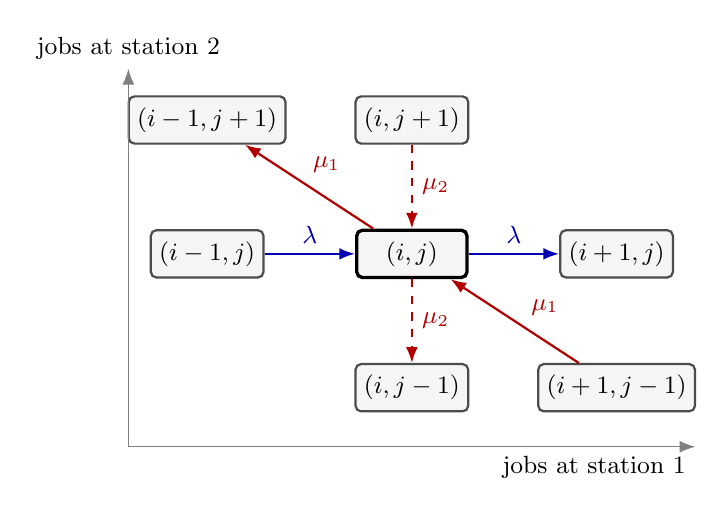
\begin{tikzpicture}[font=\small, >={Latex[length=2mm]},
  s/.style={rectangle, rounded corners=2pt, draw=gray!60!black, thick, fill=gray!8, inner sep=3pt, minimum width=14mm, minimum height=6mm}]
  \def\dx{2.6} \def\dy{1.7}
  \node[s, very thick, draw=black] (c) at (0,0) {$(i,j)$};
  \node[s] (l) at (-\dx,0) {$(i-1,j)$};
  \node[s] (r) at (\dx,0) {$(i+1,j)$};
  \node[s] (u) at (0,\dy) {$(i,j+1)$};
  \node[s] (d) at (0,-\dy) {$(i,j-1)$};
  \node[s] (ul) at (-\dx,\dy) {$(i-1,j+1)$};
  \node[s] (dr) at (\dx,-\dy) {$(i+1,j-1)$};
  % arrivals at station 1
  \draw[->, thick, blue!70!black] (l) -- node[above] {$\lambda$} (c);
  \draw[->, thick, blue!70!black] (c) -- node[above] {$\lambda$} (r);
  % service completions at station 1
  \draw[->, thick, red!70!black] (dr) -- node[above right, pos=0.45] {$\mu_1$} (c);
  \draw[->, thick, red!70!black] (c) -- node[above right, pos=0.55] {$\mu_1$} (ul);
  % service completions at station 2
  \draw[->, thick, red!70!black, dashed] (u) -- node[right] {$\mu_2$} (c);
  \draw[->, thick, red!70!black, dashed] (c) -- node[right] {$\mu_2$} (d);
  % axes
  \draw[->, thin, gray] (-3.6,-2.45) -- (3.6,-2.45) node[below left, black] {jobs at station 1};
  \draw[->, thin, gray] (-3.6,-2.45) -- (-3.6,2.35) node[above, black] {jobs at station 2};
\end{tikzpicture}
\end{document}
